\documentclass[xcolor=table]{beamer}
\usetheme[progressbar=frametitle]{metropolis}
\usepackage{appendixnumberbeamer}

\usepackage[absolute,overlay]{textpos}
\usepackage{booktabs}
\usepackage{pgf, tikz}
\usepackage{pdfcomment}
\usepackage{pgfplots}
\usepackage{hyperref}
\usepackage[utf8]{inputenc}
\usepackage{xspace}
\usepackage{color}
\newcommand{\themename}{\textbf{\textsc{metropolis}}\xspace}
\newcommand\FontImportant{\fontsize{15}{20}\selectfont}
\newcommand\FontMoyenImportant{\fontsize{14}{17}\selectfont}
\newcommand\FontPetit{\fontsize{8}{6}\selectfont}
\title{Simulation de formes réalistes de développement résidentiel, de l'échelle du bâtiment à celle de l'ensemble d'une région urbaine}
\author{Maxime Colomb}
\subtitle{\textit{Sous la direction de M. Brasebin, J. Perret \& C. Tannier}
	\\Soutenance de thèse}

\titlegraphic{\includegraphics[height=1.1cm]{Images/logoIGN.png}\hfill\includegraphics[height=1.1cm]{Images/logoThema.jpg}}

\makeatletter
\newcommand\addsectiontotoc[1]{%
  \addtocontents{toc}{%
    \protect\beamer@sectionintoc{\the\c@section}{#1}{\the\c@page}{\the\c@part}%
                                {\the\beamer@tocsectionnumber}}
}
\makeatother

\makeatletter
\newcommand{\miniscule}{\@setfontsize\miniscule{4}{5}}% \tiny: 5/6
\makeatother

\setbeamerfont*{section in head/foot}{size=\miniscule}
\setbeamercolor{section in head/foot}{parent=palette primary}

\addtobeamertemplate{frametitle}{}{%
  \begin{textblock*}{5cm}(11cm,0.1cm)
    \insertsectionnavigation{4cm}
  \end{textblock*}
}
\begin{document}

\maketitle
\section{Introduction}
\begin{frame}{Contexte : le phénomène d'étalement urbain}
	\begin{block}{}
		\begin{itemize}
			\item Répond aux souhaits d'un grand nombre de ménages
			\item Multiples effets négatifs
			\item Objectif de régulation
		\end{itemize}
		\includegraphics[height=2.8cm]{Images/consome.jpg}
		\includegraphics[height=2.8cm]{Images/sto.jpeg}
	\end{block}
	\begin{block}{}
		Dynamiques résidentielles prépondérantes %Le logement étant le principal levier de ce développement, nous nous concentrons sur le développement résidentiel
	\end{block}
\end{frame}

\begin{frame}{Contexte : documents d'aménagement réglementant l'extension résidentielle} 
	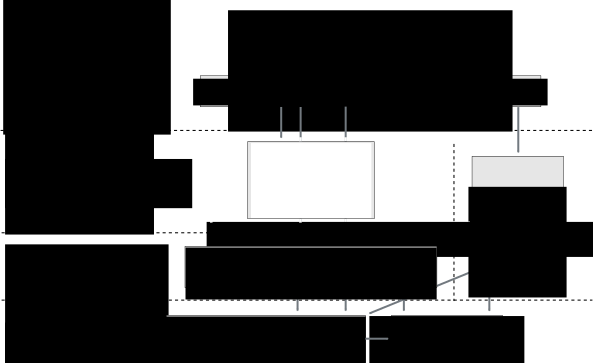
\includegraphics[width=11cm]{Images/planification-globale-Prez.png}
\end{frame}

%\begin{frame}{Objectifs principaux}
%	\begin{itemize}
%		\item Étude des effets des documents d'aménagement sur le développement résidentiel
%		\item Développer un outils pour permettre aux rédacteurs de les rendre plus efficaces
%	\end{itemize}
%\end{frame}

\begin{frame}{Enjeux : concordance des documents d'urbanisme}
	\begin{itemize}
		\item Leurs rédacteurs sont différents
		\item Leurs objectifs peuvent varier
		\item Leurs effets peuvent être contradictoires
	\end{itemize}
	\uncover<2->{	
		\begin{block}{}
			Prévoir en amont leurs effets afin d'améliorer leurs concordance et de préciser leurs effets
			%\textbf{Nécessité d'uniformiser les documents d'urbanisme et de planification pour que leurs actions soient concordantes}
		\end{block}
	}
\end{frame}

\begin{frame}{Outils d'aide à la décision pour l'aménagement}
	\begin{block}{}
		\textbf{Objectifs}\\
		Modélise un ou plusieurs phénomènes\\
		Simulations réapplicables et systématisables\\
		...
	\end{block}
	\uncover<2->{	
	\begin{block}{}
		\textbf{Utilisations}\\
		Représenter des futurs potentiels, enviables ou non\\
		Permettre de comparer plusieurs versions de document\\
		... 
	\end{block}
	}
\end{frame}

\begin{frame}{Outils d'aide à la décision pour l'aménagement}
\begin{block}{}
	\textbf{Objectifs}\\
	Modélise un ou plusieurs phénomènes\\
	Simulations réapplicables et systématisables\\
	...
\end{block}
\uncover<2->{	
	\begin{block}{}
		\textbf{Utilisations}\\
		Représenter des futurs potentiels, enviables ou non\\
		Permettre de comparer plusieurs versions de document\\
		... 
	\end{block}
}
\end{frame}

\begin{frame}{Problématique}
		Comment développer un outil permettant de simuler différents types de contraintes et à différentes échelles? 
\end{frame}

\begin{frame}{Objectifs de la thèse}
	\begin{block}{}
	Étude des \textbf{documents d'aménagements}
		\begin{itemize}
			\item représenter leurs \textbf{effets} sur le développement résidentiel
			\item Assister les aménageurs dans leurs élaborations
		\end{itemize}
	\end{block}
	\uncover<2->{
		\begin{block}{}
		Création d'un modèle de développement résidentiel afin de simuler des évolutions~:
		\begin{itemize}
			\item réaliste (respectant les règlements et les contraintes physiques et fonctionnelles)
			\item multi-échelle (d'une agglomération à la parcelle)
		\end{itemize}
	\end{block}
	}
\end{frame}




\section[Plan]{Plan de la présentation}




\begin{frame}{Plan de la présentation}
	\begin{itemize}
		\item Présentation d'\textbf{ArtiScales}
		\item Présentation des \textbf{modules} d'ArtiScales
		\item Présentation d'une \textbf{expérimentation} d'ArtiScales
	\end{itemize}
\end{frame}




\section{ArtiScales}


\begin{frame}{Caractéristiques nécessaires du modèle}
\begin{block}{}
	Création d'un modèle de développement résidentiel afin de simuler des évolutions~:
	\begin{itemize}
		\item Simuler un développement résidentiel potentiel à l'échelle de l'agglomération 
		\item Traiter différemment certains types de zones (types de communes, interdictions de construire)
		\item Simuler la construction de bâtiments (position, type de bâtiment) en fonction des contraintes réglementaires afin d'estimer les logements créées 
	\end{itemize}
\end{block}
\end{frame}

\begin{frame}{Résultats attendus}
\begin{block}{}
Afin d'assister à la rédaction des documents d'aménagements~:
\begin{itemize}
	\item Simulation de nouvelles parcelles, bâtiments, logements 
	\item Expliciter l'articulation entre les différents documents d'aménagement
	\item Calcul d'indicateurs (fonctionnels, environnementaux, morphologiques) afin d'évaluer les développements résidentiels provoqués par ces documents
\end{itemize}
\end{block}
\end{frame}

\begin{frame}{Résultats attendus}
	\uncover<2->{
	\begin{block}{}
		Différents mécanismes à différentes échelles 
	\end{block}
	\uncover<3->{
		\begin{block}{}
			Couplage de modèles de simulation~: \textbf{ArtiScales} 
		\end{block}
	}
	}
\end{frame}


\begin{frame}{ArtiScales}
	Trois différents modèles nécessaire~:
	\begin{itemize}
		\item Détection d'emplacements intéressants à urbaniser au sein de l'agglomération
		\item Recomposition du tissus parcellaire
		\item Simulation sous contraintes des bâtiments
	\end{itemize}
	\uncover<2->{
	\begin{block}{}
		Ouverts pour permettre leurs réutilisations 
	\end{block}
	}
\end{frame}

\begin{frame}{Détection d'emplacements intéressants à urbaniser}
Faire un tableau avec les avantages et les inconvénients des différentes approches
	\begin{itemize}
		\item LUTI (UrbanSim ou MobiSim)
		\item MMA (Artznete 10)
		\item Aide à la décision multi objective
		\item Automate cellulaire
	\end{itemize}
	\uncover<2->{MUP-City (Automate cellulaire avec aide à la décision multi objective)\\
	modèle stylisé
}
\end{frame}

\begin{frame}{Recomposition du tissus parcellaire}
	\begin{itemize}
		\item UrbanSimul : marché foncier mais ne permet pas d'opérations de remodelage des parcelles
		\item Algorithmes de découpages parcellaire	existent (Vanegas 12).. 
	\end{itemize}
	\begin{block}{}
		Réemploi de ces algorithmes pour développer un module : \textbf{Parcel Manager}
	\end{block}
\end{frame}

\begin{frame}{Simulation des bâtiments}
	\begin{itemize}
		\item Modèle paramètrique (Coors 2009)
		\item Modèle d'optimisation sous contrainte	: \textbf{SimPLU}
	\end{itemize}
\end{frame}

\begin{frame}{ArtiScales : Schéma}
	\includegraphics[width=3cm]{Images/mup.png}
\end{frame}




\section[MUP-City]{MUP-City et le développement résidentiel régional}




\begin{frame}{MUP-City}
	\centering{\includegraphics[width=3cm]{Images/mup.png}}
	\\
	Simulation multi-échelle du développement résidentiel 
	\begin{itemize}
		\item Considère une \textbf{région urbaine} entière
		\item Propose une \textbf{organisation spatiale locale}
		\item Met en œuvre différentes \textbf{orientations d'aménagement}
	\end{itemize}
	\includegraphics[width=6.5cm]{Images/ex-sorties-mup.png}
\end{frame}

\begin{frame}{MUP-City: entrées et sorties}
	\textbf{Entrées}
	\begin{itemize}
		\item Environnement vectoriel 
		\item Paramètres de simulation et d'orientations d'aménagements
	\end{itemize}
	\textbf{Sorties}
	\begin{itemize}
		\item \textbf{Cellules de 20m} représentant des emplacements potentiellement urbanisables
		\item Évaluations suivant des critères morphologiques et d'accessibilité
	\end{itemize}
	\begin{block}{}\centering{\includegraphics[width=9.5cm]{Images/schema_mupcity.png}}\end{block}
\end{frame}

\begin{frame}{MUP-City: analyse de sensibilité}
	\begin{itemize}

		\item 	\begin{block}{Étude des variations}
				Réplication de scénario à paramètres égaux : \alert{Robustesse}\\
				Paramètres d'entrée légèrement différents : \alert{Sensibilité}\\
				Choix scénaristiques : \alert{Analyse qualitative}

		
		\end{block}
		\item 	\begin{block}{Objectifs}
				\textbf{Fiabilité} des résultats de simulation\\
				Sélection de \textbf{configurations résidentielles} à exploiter
		\end{block}
	\end{itemize}

	\uncover<2>{\FontPetit\centering\textit{Article en préparation}}\\
	\includegraphics[width=11cm]{Images/ex-sorties-mup2.png}
\end{frame}

\begin{frame}{MUP-City: analyse de sensibilité - Exemples}

\end{frame}

\begin{frame}{Conclusion de cette étude}
	\begin{description}
		\item Systématisation des analyses par la distribution de calculs
		\item Méthodologie reproductible
		\item Sélection de plusieurs sorties à tester dans le couplage\\
	\end{description}
	\begin{block}{}\centering\includegraphics[width=11cm]{Images/exMup.png}\end{block}	
\end{frame}


\section[Parcel Manager]{Parcel Manager pour la gestion du tissus parcellaire}

\begin{frame}{Présentation du module}
THIS IS THE PART THAT EVERYBODY LOVES
\end{frame}




\section[SimPLU]{SimPLU et la simulation de bâtiments}



\begin{frame}{Présentation de SimPLU}
	\centering{\textbf{SimPLU}}
	\\
	Génère des configurations bâties en 3D
	\begin{itemize}
		\item Produit un ensemble de configurations potentiellement constructibles selon les \textbf{contraintes du PLU}
		\item Optimise certains paramètres afin de poursuivre différents \textbf{objectifs de construction}
		\item Simule le comportement d'agents constructeurs
	\end{itemize} 
	\centering{\includegraphics[width=5cm]{Images/SimpluOutput.png}}
\end{frame}

\begin{frame}{SimPLU: entrées et sorties}
	\begin{block}{Entrées}
		\begin{itemize}
			\item Parcelle au sein d'un îlot urbain
			\item Dimension et placement des ``boîtes'' simulés
			\item Fonction d'optimisation
		\end{itemize}
	\end{block}
	\begin{block}{Sortie}
		\begin{itemize}
			\item Configuration en 3D représentant un potentiel constructible
		\end{itemize}
	\end{block}
	\begin{block}
		\centering{\includegraphics[width=11cm]{Images/schema_simplu.png}}
	\end{block}		
\end{frame}

\begin{frame}{SimPLU: étude des sorties - Exemple}
	\centering{\includegraphics[width=8.5cm]{Images/simpluOutputSpace.png}}\\
	\FontPetit\centering{\textit{Explorations systématiques visant à la mise au point de de bonnes pratiques pour la création de PLU (Chapron, Brasebin, Perret et al, 2017)}}
\end{frame}





\section[Expérimentation]{Expérimentation d'ArtiScales sur l'agglomération du Grand Besançon}





\begin{frame}{Le couplage PLUCities}
%\includegraphics[width=9cm]{Images/schema-ectqg-fr.png}\\
	\FontPetit\centering{\textit{Colomb et al, 2017}}
\end{frame}


\begin{frame}{Conclusion sur ce couplage}
	\begin{block}{Conclusion sur cette expérimentation}		
		\begin{itemize}
			\item Couplage expérimental (\textit{conférence ECTQG - août 2017})
			\item \textbf{Différents scénarios} d'extension résidentielle pour un \textbf{même jeu de documents d'urbanisme}
		\end{itemize}
	\end{block}
	\begin{block}{Futurs développements}		
		\begin{itemize}
			\item Approfondir les scénarios
			\item Analyse quantitative
			\item \textbf{Exploration} des différentes configurations spatiales possibles
		\end{itemize}
	\end{block}
\end{frame}




\section{Conclusion}




\begin{frame}{Conclusion sur mes travaux de thèse}
		
\end{frame}

\begin{frame}[standout]
	\centering
	\begin{block}{}	
		\centering	
		Merci pour votre attention
	\end{block}
	\begin{block}{}
		\centering
		\textit{Everything we do is open source}\\
		\large
		\textbf{MUP-City}: \url{https://sourcesup.renater.fr/mupcity/} \\
		\textbf{SimPLU}: \url{https://github.com/IGNF/simplu3D}\\
		\textbf{PLUCities :} \url{https://github.com/ArtiScales/}  
	\end{block}
\end{frame}

\begin{frame}{Données nécessaire à l'exécution de MUP-City}
	\centering{\includegraphics[width=10cm]{Images/schemaSetData.png}}
\end{frame}
\begin{frame}{Données nécessaire à l'exécution de SimPLU}
%		\centering{\includegraphics[width=8.5cm]{Images/simplu3DNbConfigs.png}}
%	\centering{\includegraphics[width=5cm]{Images/simplumodel.png}}
\end{frame}
\end{document}


\begin{frame}{Documents de planification régionale}
Le \textbf{Schéma de Cohérence Territoriale} (SCoT) \textbf{synchronise} les politiques territoriales régionales
\begin{itemize}
	\item Territorialise la construction de logements
	\item Fixe des contraintes morphologiques et de densité
\end{itemize}
\uncover<2->{Le \textbf{Programme Local de l’Habitat} (PLH) fixe la \textbf{politique du logement}
	\begin{itemize}
		\item Précise le nombre et le type de logements prévus par communes
		\item Programme de futures opérations
	\end{itemize}
	\uncover<3>{\textbf{Relation de compatibilité entre ces deux documents}}
}
\end{frame}

\begin{frame}{Documents de planification régionale - Exemple}
\includegraphics[width=11cm]{cartes/prevision-plh.png}
\end{frame}

\begin{frame}{Documents de planification locale - Les PLU}
Le \textbf{Plan Local de l’Urbanisme (PLU)} détaille et spatialise les contraintes de constructibilité au sein d’une commune
\begin{itemize}
\item a des \textbf{effets directs sur la constructibilité} mais ne planifie pas la construction 
\item \textbf{donne un cadre} pour la création de programmes de construction de logements \textit{(OAP, ZAC, ZAD)}
\item se compose en partie d'un \textbf{zonage} et d'un \textbf{règlement}
\end{itemize}
\end{frame}	

\begin{frame}{Application d'un PLU - Le zonage}
\begin{columns}[T]
\begin{column}[T]{7cm}
Zones générales et sous-zones particulières
\begin{itemize}
\item \alert{Naturelles} \textbf{(N)} \emph{non constructibles}
\item \alert{Agricoles} \textbf{(A)} \emph{non constructibles}
\item \alert{Urbanisées} \textbf{(U)}
\item \alert{À Urbaniser} \textbf{(AU)}
\end{itemize}
\end{column}
\begin{column}[T]{4cm}
\begin{textblock*}{6cm}(7.5cm,1.5cm)
\includegraphics[width=5cm]{cartes/plu-roche.png}
\end{textblock*}	
\end{column}
\end{columns}

\end{frame}

\begin{frame}{Application d'un PLU - Le règlement}
\begin{columns}[T]
\begin{column}[T]{5cm}
Pour chaque sous-zone : 
\begin{itemize}
\item Articles 1, 2 : restrictions d’\textbf{usage du sol}
\item Articles 6, 7, 8 : \textbf{position des bâtiments} relativement aux autres bâtiments, aux limites de parcelles ou à la voirie
\item Article 10 : \textbf{hauteur maximale}
\item Article 11 : \textbf{aspect extérieur}
\end{itemize}
\end{column}
\begin{column}[T]{5.5cm}
\centering
\includegraphics[width=6cm]{Images/codesplu.png}
\\
\textit{Exemple de prescriptions graphiques (PLU de Strasbourg)}
\end{column}
\end{columns}
\end{frame}

\begin{frame}{Opportunités pour l'IGN}
%	\centering{\includegraphics[width=4cm]{Images/franceGPU.png}}\\
%	\FontPetit{\textit{Dépôt des PLU sur le GPU}}
\begin{itemize}
	\item Définition de données adaptées à la simulation des évolutions
	\item Proposition de service aux acteurs de la planification sur l'ensemble du territoire français
	\item Certification de la robustesse du processus de simulation relativement à la qualité des données
\end{itemize}
\end{frame}